\documentclass[standalone, version=2.0]{huangfusl-template}
\begin{document}
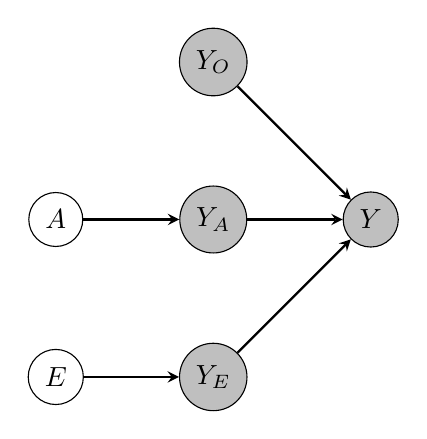
\begin{tikzpicture}
    \node[circle, draw] (A) at (-2, 0) {$A$};
    \node[circle, draw] (E) at (-2, -2) {$E$};
    \node[circle, draw, fill=gray!50!white] (YE) at (0, -2) {$Y_E$};
    \node[circle, draw, fill=gray!50!white] (YA) at (0, 0) {$Y_A$};
    \node[circle, draw, fill=gray!50!white] (YO) at (0, 2) {$Y_O$};
    \node[circle, draw, fill=gray!50!white] (Y) at (2, 0) {$Y$};

    \foreach \i in {A, E} {
        \draw[-stealth, thick] (\i) -- (Y\i);
        \draw[-stealth, thick] (Y\i) -- (Y);
    }
    \draw[-stealth, thick] (YO) -- (Y);
\end{tikzpicture}
\end{document}